\documentclass[main.tex]{subfiles}
\begin{document}

In the following subsections, we will reproduce some of the results mentioned
in Section \ref{sec:theor_searching} using \texttt{QWAK}, displaying how the
package allows the user to easily simulate the search problem for different
structures.


\subsubsection{Complete Graph}

To use QWAK for searching, we need to define a graph for the search space, and
the targets are marked elements, specified as a list of weighted node indices.
For a complete graph, the optimal transition rate is \(\gamma = \frac{1}{n}\),
resulting in a search time of \(\mathcal{O}(\sqrt{N})\), comparable to Grover's
algorithm \cite{farhi1996, childs2004}.

\begin{lstlisting}[style=code,escapeinside={__}]
n = 200
t = (np.pi/2) * np.sqrt(n)
gamma = 1/n
init = list(range(0,n))
graph = nx.complete_\textunderscore_graph(n)
qw = QWAK(graph,gamma=gamma,markedElements=[(n//2,-1)],
                                       laplacian=False)
qw.runWalk(t,initStateList=init)
\end{lstlisting}

Firstly, we initialize the \texttt{QWAK} with the desired simulation
parameters, so that we can calculate the search problem via the runWalk method.
Because we created the object with a list of marked elements, the Hamiltonian
of the method will be described as in equation
\eqref{eq:searchHamiltonian}.\par

\begin{figure}[!h]
    \centering
    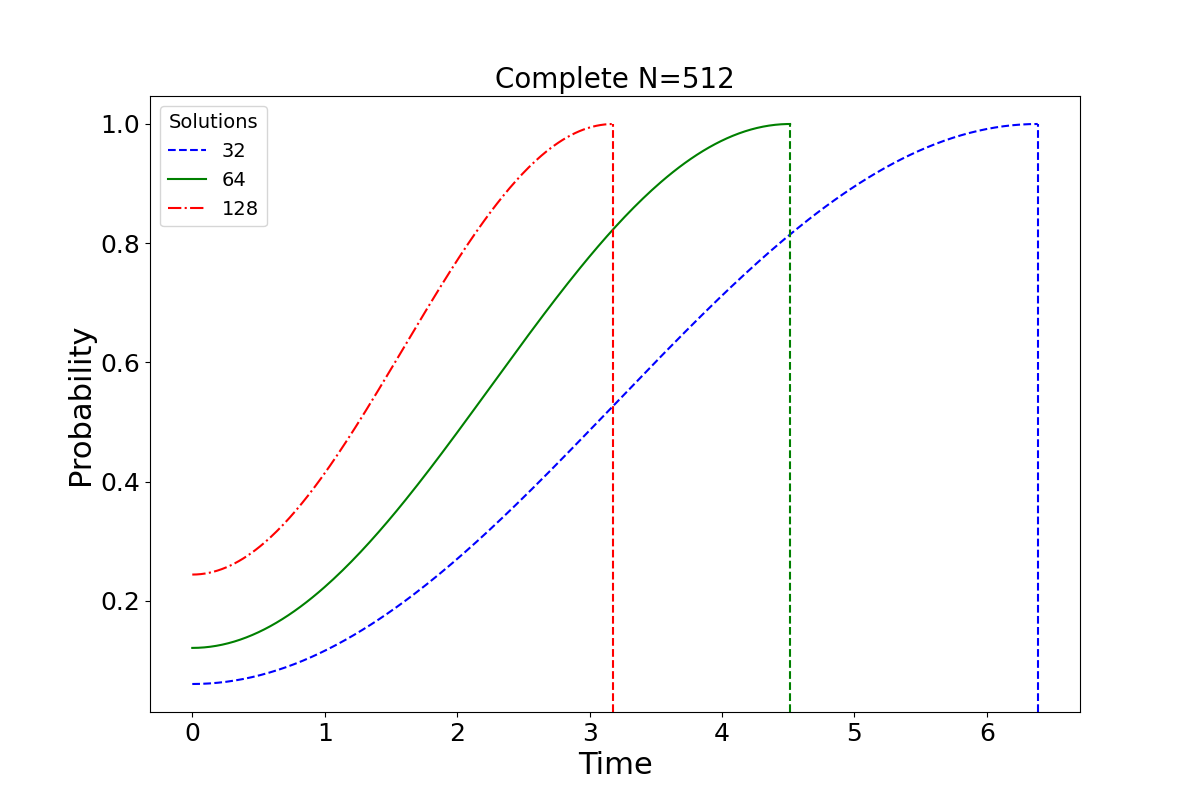
\includegraphics[scale=\mysinglefigurescale]{img/QWAK/CompleteSearch/completePlot_N512_NWALKS3_S200.png}
    \caption{Total probability of marked elements in a CTQW search on a
    complete graph of size $N=512$, as a function of time, with varying number
    of solutions.} 
    \label{fig:multipleElementCompleteGraph}
\end{figure}

The optimal time for the search problem also depends on the number of solutions
\cite{boyer1996,Lugao2022}, and Fig. \ref{fig:multipleElementCompleteGraph}
presents the evolution of sum probability of all the marked elements. The
utility functions needed to plot this figure are available in the package. 

\begin{lstlisting}[style=code]
markedElements = [(n//2,-1),(n//2+1,-1)]
t = (np.pi/2) * np.sqrt(n/len(markedElements))
\end{lstlisting}

To search for multiple elements, we simply extend the \texttt{markedElements}
list and fine-tune the optimal evolution time. The aforementioned figure
demonstrates that as the number of marked elements increases, the time required
to reach maximum probability decreases. Specifically, when we mark $
\frac{1}{4} $ of the total elements, the walk evolves optimally in time $\pi$.
This scenario is analogous to the \textit{single-shot Grover algorithm}, where
the highest probability for finding the solution is achieved in just one step.

\subsubsection{Hypercube}

The $n$-dimensional hypercube is a graph of $N=2^n$ vertices, where two
vertices will be connected if their binary representation differs only in a
single bit to the other. The evolution of the search problem over this
structure presents a sharp transition at a critical value of $\gamma$ \cite{childs2004}, given by

\begin{equation}
    \gamma_{opt} =\frac{1}{2^n} \sum_{r=1}^n\left(\begin{array}{l}
        n \\
        r
        \end{array}\right) %\frac{1}{r}=\frac{2}{n}+O\left(n^{-2}\right)
\end{equation}

Here, we attempt to showcase that the maximum probability of the solution is
indeed sensitive to the transition rate. For this purpose, we create a
\texttt{QWAK} object for a range of $\gamma$ values, and then we evolve the
walk in a time interval with the \texttt{runMultipleWalks} function.

\begin{lstlisting}[style=code,escapeinside={__}]
n = 9
gamma = gamma_\textunderscore_hypercube(n)
graph = nx.hypercube_\textunderscore_graph(n)
N = 2**n
t = (np.pi/2) * np.sqrt(N)
init = list(range(0,N))
tList =  list(range(0,2t))
probDistMat = []
for gamma in gammaList:
    qw = QWAK(graph,gamma=gamma,initStateList=init,
                        markedElements=[(N//2, -1)])
    qw.runMultipleWalks(tList)
    probDistMat.append(qw.getProbDistList())
\end{lstlisting}

The distribution matrix is composed of lists of
\texttt{ProbabilityDistribution} objects, for each value of $\gamma$. We now
generate a plot to visualize the search process and the effect of different
values of $\gamma$ on the probability of finding the marked element. The plot
is shown in Figure \ref{fig:hypercubeSearch}, obtained with auxilary functions
available in the notebook.

\begin{figure}[!h]
    \centering
    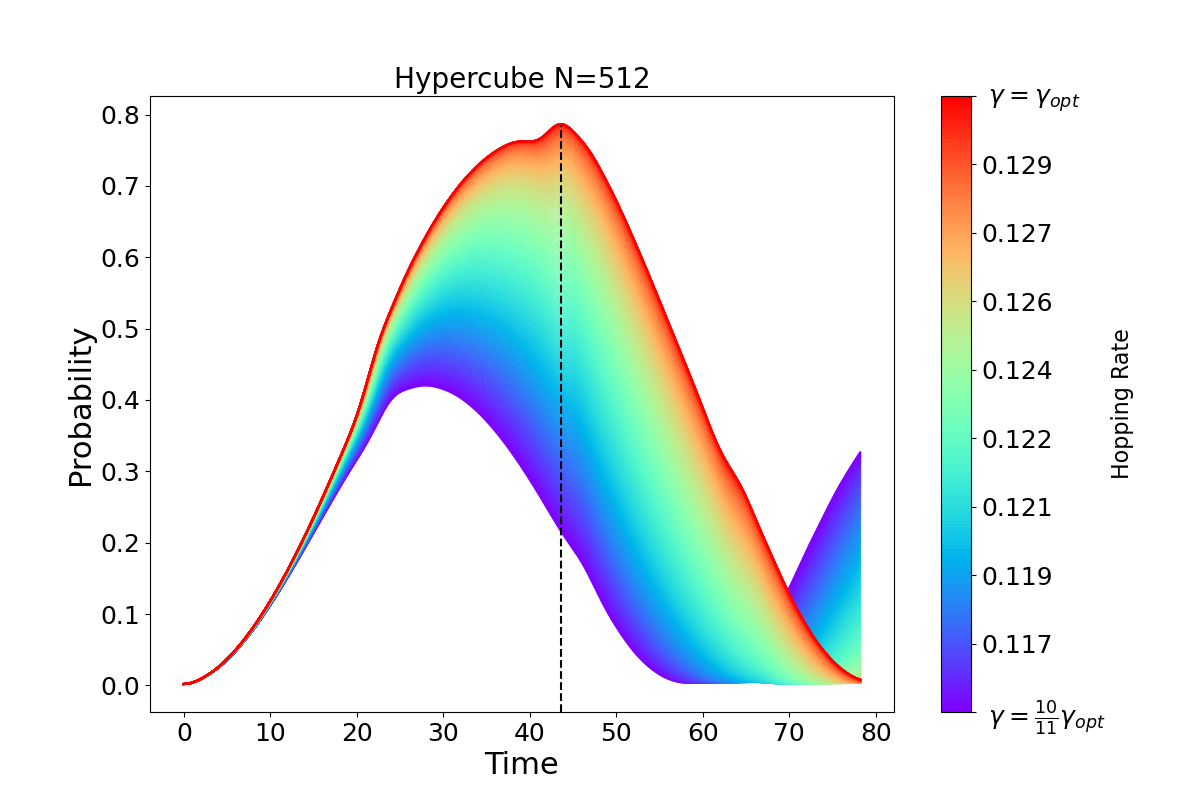
\includegraphics[scale=\mysinglefigurescale]{img/QWAK/HypercubeSearch/hypercubePlot_N512_S200_GMIN0.117_TMAX78.png}
    \caption{Total probability of marked elements in a CTQW search on a hypercube
    graph of size $N=512$, as a function of time, for a range of transition
    rate values represented in the color bar.} 
    \label{fig:hypercubeSearch}
\end{figure}

We can see from the plot that despite having a very narrow range of transition
rate values, $\gamma_{opt}$ does indeed reach maximum probability within time
that scales with $\mathcal{O}\sqrt{N}$.

\subsubsection{Erdős-Rényi model}

As a final example, we will examine the search problem on a more general
collection of random graphs. In the Erdős-Rényi (ER) model, a graph is
generated with a fixed number of nodes, connecting each pair of nodes with a
probability $p$. This leads to graphs with diverse levels of connectivity,
dependent on $p$. Existing research shows that CTQWs are optimal for
searching on most such graphs, given certain conditions~\cite{chakraborty2016}.
To further explore this, we will conduct simulations on ER graphs with varying
connection probabilities.

\begin{lstlisting}[style=code,escapeinside={__}]
N = 500
t = (np.pi/2) * np.sqrt(N)
samples = 200
pList = np.linspace(0.01, 0.5, samples)
graphList = [nx.erdos_\textunderscore_renyi_\textunderscore_graph(N, p) for p in pList]
\end{lstlisting}


Next, we initialize a QWAK object for each graph in the list and set a
transition rate of $\gamma = \frac{1}{N p}$. We will store the probability
distributions in a matrix for further analysis.

\begin{lstlisting}[style=code,escapeinside={__}]
initSL = list(range(0, N))
tList = np.linspace(0, 2t, samples)
probDistMat = []
for graph,pVal in zip(graphList,pList):
    gamma = 1/N*pVal
    qw = QWAK(graph,gamma=gamma,initStateList=init,
                       markedElements=[(N//2,-1)])
    qw.runMultipleWalks(timeList=tList)
    probDistMat.append(qw.getProbDistList())
\end{lstlisting}

Finally, we can visualize the results in Fig. \ref{fig:ERSearch} by
generating a heatmap plot, with the connection probabilities on the x-axis as a
function of time in the y-axis. The color intensity represents the
maximum probability of finding the marked element at each combination of
parameters.

\begin{figure}[!h]
    \centering
    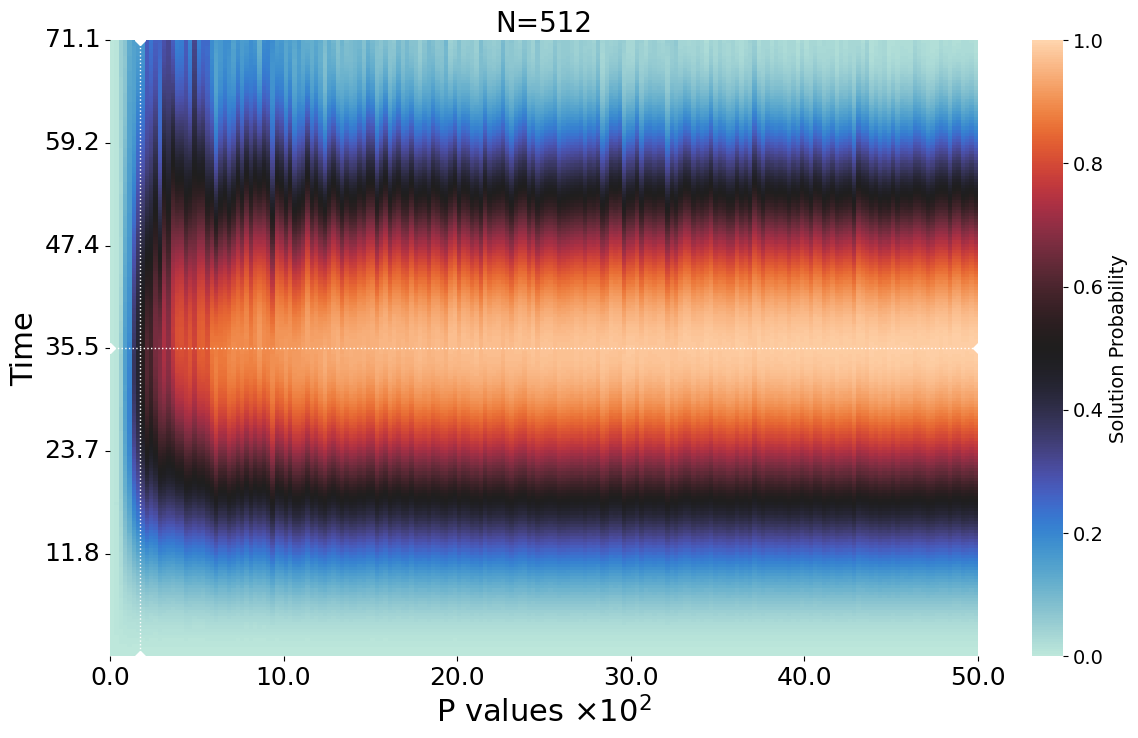
\includegraphics[scale=\mysinglefigurescale]{img/QWAK/ERSearch/heatMapPlot_N512_NGRAPHS40_S200_PMAX0.5.png}

    \caption{Heatmap of the total probability of marked vertices in a CTQW search on
    Erdős–Rényi graphs of size $N=512$, as a function of time and connection probability.}
    

    \label{fig:ERSearch}
\end{figure}

When the value of $p$ in a graph exceeds the percolation threshold of
$p=\frac{\log{N}}{N}$, the graph is almost certainly connected
\cite{chakraborty2016}.  The figure highlights this threshold with a vertical
line and shows that the search process achieves high solution probabilities
above it, in time $\mathcal{O}(\sqrt{N})$. For each value of $p$, $40$
different graphs were generated in order to calculate the average solution
probability.

\end{document}
